% !TEX encoding = UTF-8 Unicode
%%%%%%%%%%%%%%%%%%%%%%%%%%%%%%%%%%%%%%%%%%%%%%%%%%%%%%%%%%%%%%%%%%%%%%%%%%%%%%%%%%%%%%%%%%%%%%%%%%%%%%% 
%%
%%  This file is asmeconf-template.tex, a LaTeX template to format ASME Conference papers according to
%%  the requirements on ASME's conference web pagess, and including hypertext support for the pdf.
%%
%%  This file is version 1.45 dated 2025/11/10
%%  
%%  As of version 1.11, this template defaults to ASME's newer conference guidelines first posted July 2019.
%% 			Those guidelines changed the author block formatting to be inline. 
%%			If you prefer the traditional grid format, use the class option [grid].
%%			Nomenclature now follows the abstract, and the abstract text is set in italics.
%%
%%  Author: John H. Lienhard, V
%%          Department of Mechanical Engineering
%%          Massachusetts Institute of Technology
%%          Cambridge, MA 02139-4307 USA
%%
%%  Class options include:
%%
%%          * An option to use the traditional grid arrangement of author names, [grid].  
%%			*	 With this option, line breaks (\\) may be inserted into the address as needed. 
%%			*	 Author names that include commas should be enclosed in braces, e.g.,  {Joseph L. Smith, Jr.}.  
%%			*	 Authors may be grouped above a single affiliation using braces, e.g., {Henry Tudor, Catherine Parr}.
%%
%%          * An option to balance the heights of columns on the last page, [balance]. 
%%
%%          * An option to include line numbers, [lineno]. You must *run twice* for proper placement of the line numbers. 
%%			*	 The lineno package does not number titles, footnotes, captions, or tables.
%%          *    This option will disable balancing column height on final page if that option has been invoked.
%%          *    The lineno package won't always number the lines preceding displayed math in a paragraph because
%%          *    paragraph has not ended.  See that package's documentation for macros to address this problem, or
%%          *    just leave a blank line above the displayed equation while you are editing and then remove the 
%%          *    blank line along with [lineno] option when you move to your final version.
%%
%%			* An option not to use a boldface font for caption text, [unboldcaption]
%%
%%          * Options to: 	omit the ASME copyright footer, [nofoot]; 
%%			*				use government employee copyright notice,      [govt];
%%			*				use government contractor copyright notice,    [contractor];
%%			*				use copyright notice for some gov't employees, [somegovt];
%%			*				omit the conference headers on the titlepage,  [nohead]
%%
%%			* Option to use LuaLaTeX **without** unicode-math and fontspec, [nofontspec]
%%
%%          * Math options from M. Sharpe's newtxmath package: upright integrals [upint]; 
%%          *    [varvw] for a v and w that are better distinguished from Greek nu; and also 
%%          *    [subscriptcorrection, smallerops, varg, frenchmath, varbb, cmbraces, slantedGreek,...] 
%%			* 	 See newtx documentation for descriptions (at CTAN: https://www.ctan.org/pkg/newtx, v1.744 or higher is best).
%%			*	 newtx is not loaded with lualatex unless the [nofontspec] option is used.
%%
%%          * An option to allow hyphenation of the typewriter font [hyphenate], from the inconsolata package (pdfTeX only).
%%          *    Hyphenation is normally suppressed for a typewriter (monospaced) font because those are often used for code.
%%			*	 To replace the default variable word spacing by monospacing, use the option [mono].
%%			*	 To get a zero without a slash, use [var0]
%%
%%			* PDF/A compliance:  Since 2022, LaTeX has included support for PDF/A, through the \DocumentMetadata{..} command.
%%
%%          * Options (used by the babel package) to include passages in languages other than English (e.g., a translation 
%%			*    of the abstract).  See Appendix C for details.
%%			*    	pdftex: Appropriate scripts will be loaded if you call the class options [greek], [russian], or [vietnamese].
%%			*    
%%			*    	lualatex: Language support is most extensive when running LuaLaTeX, which automatically loads fontspec.
%%			*		Non-Latin scripts require the [loadscripts] option, see Appendix C. 
%%			*	 	Be aware that you might need to install additional fonts for some languages.
%%			 
%%  The use of commands defined or modified by the asmeconf class is illustrated throughout this file. In particular, 
%%  ASME requires capitalized section headings, and as a result some care is needed when using macros in section headings,
%%  as also illustrated below.
%%
%%  Use an **up-to-date and complete** installation of LaTeX, such as TeX Live 2025 or later. 
%%		LaTeX formats earlier than 2022 are not fully supported.
%%
 %=========================================================
%% 
%% LICENSE: 
%%
%% Copyright (c) 2025 John H. Lienhard
%%
%% Offered under the MIT license: https://ctan.org/license/mit 
%%
%%%%%%%%%%%%%%%%%%%%%%%%%%%%%%%%%%%%%%%%%%%%%%%%%%%%%%%%%%%%%%%%%%%%%%%%%%%%%%%%%%%%%%%%%%%%%%%%%%%%%%% 

%%  RECOMMENDED pdf management code.
%%  This code was added to the LaTeX kernel in June 2022.
%% 		See https://www.latex-project.org/news/latex2e-news/ltnews35.pdf
%%  If you have problems with these lines, you can comment them out or, better, update your LaTeX format.

\DocumentMetadata{
	lang		= eng-US, 	% default
	pdfstandard	= A-3u,		% A-2b, A-2u, A-3b, A-3u. Check that your figures also meet the standard you choose.
	pdfversion	= 1.7, 		% an older version of PDF, but very widely supported
%	pdfversion  = 2.0, 		% default for LaTeX. Version 2.0 supports tagged PDF.
%	pdfstandard = { ua-2 , a-4f }, % run with lualatex and use a very recent LaTeX format (e.g., 2025/11/01)
%	tagging 	= on, 		% for producing tagged pdf
}

%%%%%%%%%%%%%%%%%%%%%%%%%%%%%%%%%%%%%%%%%%%%%%%%%%%%%%%%%%%%%%%%%%%%%%%%%%%%%%%%%%%%%%%%%%%%%%%%%%%%%%%

%% CLASS OPTIONS are described above. Change the options given below to meet your needs.
%% 
%%	 	NB: Remove the [colorlinks] option before *final* submission to ASME, to get black text for printing,
%%			but keep that option for electronic use.
%%
%%		NB: If you are not using the language options, * remove * them (together with Appendices C and D).
%%			Greek, cyrillic languages, and vietnamese if used, must be named as \documentclass options under pdftex.
%%			Spanish, german, and many others, if used, do not need to be named when the babel package is dated 2024 or later.
%%
%%		NB: the mathalfa option was dropped in v1.41; load the mathalpha package in your preamble instead.

\documentclass[colorlinks,upint,subscriptcorrection,varvw,hyphenate,balance]{asmeconf} % pdftex
\usepackage{tikz}
\usetikzlibrary{arrows.meta,positioning,calc,shapes.geometric}
\usepackage{placeins}
\usepackage{float}

%\documentclass[colorlinks,upint,subscriptcorrection,varvw,balance,loadscripts,german,vietamese]{asmeconf} % lualatex

%%%%%  pdf metadata  %%%%%%%%%%%%%%%%%%%%%%%%%%%%%%%%%%%%%%%%%%%%%%%%%%%%%%%%%%%%%%%%%%%%%%%%%%%%%%%%%%

\hypersetup{%
	pdfauthor={John H. Lienhard},									  % <=== change to YOUR name
	pdftitle={ASME Conference Paper LaTeX Template},                  % <=== change to YOUR pdf file title
	pdfkeywords={ASME conference paper, LaTeX template, BibTeX style},% <=== change to YOUR pdf keywords
	pdfsubject = {Describes the asmeconf LaTeX template},			  % <=== change to YOUR subject
%	pdfurl={https://ctan.org/pkg/asmeconf},% may delete
%	pdflicenseurl={https://ctan.org/pkg/asmeconf},% may delete
}
% If an author name or the title include a comma, enclosed it in braces, e.g., pdfauthor{John Forbes Nash{,} Jr.}


%%%%%%%%%%%%%%%%%%%%%%%%%%%%%%%%%%%%%%%%%%%%%%%%%%%%%%%%%%%%%%%%%%%%%%%%%%%%%%%%%%%%%%%%%%%%%%%%%%%%%%%

\allowdisplaybreaks % from amsmath package, allows multiline equations to break across pages (delete if not wanted)
					% using \\* instead of \\ will prevent specific lines from being pagebreaks.

% logos used in this document
\newcommand*\pdfTeX{pdf\TeX}    
\newcommand*\LuaLaTeX{Lua\LaTeX}
\newcommand*\BibTeX{Bib\TeX}

\begin{document}

% Change these fields to the right content for your conference.
% You can comment these out if for some reason you don't want a header.
% Use title case for the conference name (first letters capitalized), not all capitals

\ConfName{Proceedings of the ASME 2026\linebreak International Design Engineering Technical Conferences \&\linebreak Computers and Information in Engineering Conference}
\ConfAcronym{IDETC-CIE 2026}
\ConfDate{August 23--26, 2026}
\ConfCity{Houston, TX, USA}
\PaperNo{DETC2026-XXXX}

% Units of measure (e.g., cm) and other specialty lowercase terms in the title should be 
%   enclosed in \NoCaseChange{...} to maintain lower case type.
%   The rest of the title will automatically be set in all capital letters.
%
%	\title{Place Title Here: Place Subtitle After Colon} 

\title{Reliable Natural-Language to SysMLv2 Translation via Validator-Driven Iterative Refinement} % <=== replace with YOUR title
 
%   Put author names into the order you want. Use the same order for affiliations.
%   \affil{#} tags the author's affiliation to the address in \SetAffiliation{#}.
%   No space between last name and \affil{#}, separate names with commas.
%
%	For a sole author or a single affiliation for all authors, {#} may be left empty, i.e. \affil{} and \SetAffiliation{} (but not with [grid] option!)
%
%   \CorrespondingAuthor{email} follows that author's affiliation, no spaces before or after 
%   If multiple corresponding authors, put both email addresses in the same command and place after both authors.
%
%   \JointFirstAuthor, if applicable, follows the affiliation of the relevant authors, no spaces.

\SetAuthors{%
    Chance LaVoie\affil{1}\CorrespondingAuthor{chancel@cmu.edu},
    Eladio Andujar Lugo\affil{1},
    Levent Burak Kara\affil{1}
}

\SetAffiliation{1}{Department of Mechanical Engineering, Carnegie Mellon University, Pittsburgh, PA 15213 USA}
%   Note: You can force a line break in the address using \\ 

%	To switch from inline author names to gridded names, use the [grid] option.

\maketitle

%%% Use this footnote for tracking various versions of your draft. Change text to suit your own needs. 
%%% \date{..} calls the same command. 
\versionfootnote{Documentation for \texttt{asmeconf.cls}: Version~\versionno, \today.}% <=== Delete before final submission.

%%% Change the following to your keywords.  Keywords are automatically printed at the end of the abstract.
%%% This command MUST COME BEFORE the end of the abstract.
%%% If you don't want keywords, leave the argument of \keywords{} empty (or use the abstract* environment)

\keywords{SysMLv2, model-based systems engineering, large language models, validator-in-the-loop, natural language to model translation, syntactic validity}

%%%%%  End of fields to be completed. Now write your paper. %%%%%%%%%%%%%%%%%%%%%%%%%%%%%%%%%%%%%%%%%%%


%%%%%  ABSTRACT  %%%%%%%%%%%%%%%%%%%%%%%%%%%%%%%%%%%%%%%%%%%%%%%%%%%
%%
%% Abstract should be 200 words or less
\begin{abstract}

\end{abstract}

%%%%%%%%%  BODY OF PAPER %%%%%%%%%%%%%%%%%%%%%%%%%%%%%%%%%

\section{Introduction}
Model-Based Systems Engineering (MBSE) replaces document-centric workflows with model-centric engineering, where formal artifacts carry requirements, structure, behavior, and verification intent across the lifecycle~\cite{estefan2007mbseSurvey,madni2018mbse,incoseMbseInitiative2025,sebokMBSE2025}. By making the model the primary technical source, MBSE reduces cross-document reconciliation overhead and improves traceability under change~\cite{madni2018mbse,incoseSEVision2035}.

SysMLv2 strengthens this transition by standardizing a formal language with complementary textual and graphical representations and machine-readable artifacts under OMG~\cite{omgSysMLv2Spec2024,omgSysMLv2About2025,omgSysMLv2FinalAdoption2025}. In practice, the same model can be authored as text, rendered visually, and exchanged across tools with less ambiguity. Because SysMLv2 is formal and textual, model construction is scriptable.

This scriptability, combined with the recent rise of LLMs in engineering practice, creates a concrete opportunity for automated SysMLv2 modeling workflows. LLM-based pipelines can generate candidate models directly from natural-language inputs.

Software engineering provides encouraging precedent: controlled and field studies report substantial productivity gains from LLM-assisted generation, including 55.8\% faster task completion, 26.08\% higher weekly completed tasks in enterprise randomized deployments, and measurable increases in pull-request throughput~\cite{peng2023copilot,cui2025highSkilled,demirer2024fieldCopilot}. These results suggest that integrating generation into everyday tool use can materially accelerate engineering iteration.

The analogous opportunity in MBSE is to automate low-value model authoring steps while increasing modeling velocity. If natural-language prompts can be converted into \emph{production-validator--accepted} SysMLv2, teams can spend less effort on syntax correction and more effort on architecture and verification reasoning.

Motivated by this potential, recent SysMLv2 generation systems have moved beyond unreliable one-shot prompting toward structured generation workflows~\cite{bouamra2025systemp,cibrian2025sysmlagent}. SysTemp uses a template-first multi-agent design centered on a \textit{TemplateGeneratorAgent} and a \textit{ParserAgent}. A Jinja2-based template tool first builds a structured SysMLv2 skeleton, then a writer agent fills in content while parser feedback guides iterative correction~\cite{bouamra2025systemp}. By contrast, the 2025 \emph{Computers in Industry} framework organizes generation as an agentic loop with a RAG-based context engine and a validation engine, with ANTLR-based grammar validation as the syntax gate~\cite{cibrian2025sysmlagent}. In that framework, the context engine retrieves semantically similar natural-language prompt and SysML file pairs and exposes them to the LLM as context~\cite{cibrian2025sysmlagent}. Both approaches rely on context-free grammar (CFG) parsing as the primary basis for syntactic validation and as the primary acceptance metric.

In parallel, SysMBench has established a common benchmark for evaluating natural-language--to--SysML generation quality, especially on semantic alignment criteria~\cite{jin2025sysmbench}. Read together, the current state of the art suggests that generating SysMLv2 from natural language that passes grammar-parser checks is feasible.

Grammar parsability guarantees structural conformance to SysMLv2 context-free syntax: valid token ordering, balanced delimiters, and production-rule-compliant declarations. It does \emph{not} guarantee production validation acceptance, because industrial validators enforce additional model-wide constraints such as name resolution, type consistency, ownership/composition rules, multiplicity constraints, and cross-reference integrity. Therefore, parser-passing outputs provide no assurance that they will be accepted by a production modeling environment for downstream use, including visualization, semantic validation, simulation, and optimization. Without acceptance under a full industrial validator, such models remain unusable in practice. In an auxiliary repository demonstration, we show ten distinct cases that pass SysML ANTLR parsing but fail production validation, empirically reinforcing this distinction~\cite{antlrVsSysideDemo2026}. The critical gap is reliable generation of \emph{production-validator--accepted} SysMLv2 from arbitrary natural-language prompts.

To close this gap, we instantiate a generate--verify--refine workflow in which candidate SysMLv2 models are iteratively evaluated against a production validation backend and revised until acceptance. This paradigm is not novel in itself. It draws from established traditions in formal methods and inductive synthesis, where candidate artifacts are proposed, evaluated by an external oracle, and corrected using deterministic feedback from that oracle~\cite{clarke2000cegar,solarlezama2008thesis,jha2010ogis,alur2013sygus}. Our contribution is to operationalize this verification-driven pattern for natural-language--to--SysMLv2 generation under industry-facing acceptance criteria.

Related work in code generation has already demonstrated the technical value of iterative verifier-in-the-loop refinement. Wang et al.\ show that deterministic compiler diagnostics can be used as structured correction signals in multi-stage neural code generation, improving acceptance of generated programs under executable checks~\cite{wang2022compilable}. Grubi{\v{s}}i{\'c} et al.\ similarly use compiler feedback to iteratively refine LLM outputs, treating validator responses as an explicit control signal for subsequent generations~\cite{grubisic2024compiler}. Taken together, these works establish the core mechanism we rely on: generate a candidate, evaluate it with a deterministic backend, feed diagnostics back into the next iteration, and repeat until the validator reports no remaining errors.

We apply this principle directly to MBSE. Our framework places a production SysMLv2 syntax validator, SysIDE~\cite{sensmetry2024syside}, in the loop as a deterministic oracle, and generation proceeds until zero-error acceptance is achieved under that validator. At convergence, the resulting model is production-ready and operational within the modeling environment---loadable, renderable, analyzable, and suitable for downstream verification workflows. By elevating production-validator acceptance to the convergence criterion, SysMLv2 generation moves from syntactic plausibility to deployable modeling infrastructure, establishing a practical foundation for Copilot-like support in MBSE workflows.

\section{Related Work --- NEEDS A LOT OF WORK -- CHANCES LOWEST PRIORITY}

Our review focuses on prior efforts in automated SysML v2 generation, grammar-constrained structured synthesis, and validator-guided iterative refinement, with an emphasis on approaches addressing reliable syntactic correctness in low-data modeling languages.

\subsection{LLM-Based SysML v2 Model Generation}
Recent work has explored using large language models to generate SysML v2 models from natural language. Bouamra et al.~\cite{bouamra2025systemp} propose SysTemp, a multi-agent framework that decomposes generation into requirement extraction, template-based skeleton construction, and grammar-level parsing feedback. Two specialist agents structure the flow: a \textit{TemplateGeneratorAgent} uses a Jinja2-backed template tool to construct a syntactically organized SysMLv2 skeleton, and a \textit{ParserAgent} validates the generated text against formal SysMLv2 grammar and returns diagnostics to a writer agent for iterative repair~\cite{bouamra2025systemp}. This work demonstrates that structural scaffolding and agent decomposition improve grammar conformity in sparse-data settings, with syntactic acceptance anchored to context-free grammar (CFG) parsing. However, syntactic correctness is defined at the grammar level and convergence is reported empirically rather than enforced as a termination invariant.

Cibrián et al.~\cite{cibrian2025sysmlagent} introduce a distinct agentic architecture in \emph{Computers in Industry}: generation is orchestrated in an agentic loop with a RAG-based context engine and a validation engine (for grammar-level checking), using ANTLR-generated CFG parsing as the syntactic acceptance mechanism. Their context engine retrieves semantically similar natural-language and SysML exemplar pairs to condition generation~\cite{cibrian2025sysmlagent}. Their approach reports 100\% syntactic validity across 20 curated prompts under grammar-level parsing. While this represents a significant advance in structured generation reliability, correctness is enforced through grammar parsing rather than full production validation. Because grammar-level validation ensures context-free structural conformity but does not enforce full static semantics under a production modeling environment, grammar-valid models may still fail production validation in practice.
Together, these efforts establish that iterative validation substantially improves syntactic success in SysML v2 generation. However, prior systems define correctness primarily at the grammar level and evaluate on limited scenario sets. For industry use, the unresolved gap is generalizable \emph{production-validator--accepted} syntactic correctness across diverse prompts. An additional gap is retrieval dependence: pipelines that require semantically similar NL-SysML exemplars may be less generalizable when comparable examples are sparse or unavailable. Our work builds on these insights while shifting the correctness oracle from grammar parsing to a production SysMLv2 validator and scaling evaluation to benchmark-level scenarios.

\subsection{Grammar-Constrained and Template-Based Structured Synthesis}

Structured synthesis approaches aim to reduce hallucinations in LLM output by constraining generation via templates or grammar rules. SysTemp~\cite{bouamra2025systemp} explicitly uses a template generator based on Jinja2 to construct syntactically compliant model skeletons prior to completion. Grammar-constrained decoding and post-generation parsing similarly reduce token-level structural invalidity.

While grammar validation ensures adherence to context-free rules, it does not enforce type resolution, cross-reference integrity, constraint satisfaction, or production modeling environment compatibility. Thus, grammar-valid artifacts may remain unusable within industrial MBSE workflows. Concretely, a model such as \texttt{port p: UndefinedType;} can be grammar-parsable yet fail production validation because the referenced type is unresolved; conversely, a missing delimiter (e.g., omitted semicolon) fails parsing before production validation semantics are even checked. Our approach differs by treating grammar conformity as necessary but insufficient and requiring full production validation acceptance prior to termination.

\subsection{Validator-in-the-Loop and Verifier-Guided Generation}

Prior work in neural code generation has explored leveraging compiler diagnostics to improve the compilability of model outputs. For example, Wang et al.~\cite{wang2022compilable} propose a multi-stage refinement framework that uses compiler feedback to iteratively revise generated programs and increase compilation success rates. Such approaches demonstrate that deterministic compiler signals can serve as effective supervisory feedback in programming-language settings. However, these systems operate in mature programming ecosystems and treat compilation success as an empirical objective rather than as a structural termination invariant.

Beyond compiler-feedback approaches in code generation, iterative generation guided by deterministic verifiers has also been studied under counterexample-guided inductive synthesis and execution-based refinement paradigms. Grubišić et al.~\cite{grubisic2024compiler} demonstrate that LLVM compiler feedback can serve as a supervisory signal for refining LLM-generated intermediate representation. Their work shows that deterministic compilation signals constrain output space and improve structural validity in programming languages.

While these approaches establish the feasibility of compiler-aware refinement in software domains, they differ in both objective and context from model-based systems engineering. Compiler feedback in such systems is typically used to improve optimization quality or increase compilation probability, rather than to enforce strict termination conditions. Moreover, these methods operate in programming languages with extensive training corpora and stable ecosystems.

In contrast, our work applies validator-in-the-loop refinement to SysMLv2, a newly standardized modeling language with sparse representation in LLM training data and strict production-validation requirements. Rather than treating validation results as heuristic feedback, we enforce zero-error acceptance under a production SysMLv2 validator (invoked via \texttt{syside check}) as a termination invariant. This elevates syntactic correctness from an empirical metric to a property guaranteed by construction, aligning generation reliability with production MBSE modeling-environment criteria rather than grammar-level approximations.


\section{Methodology}

\subsection{Study Objective and Paired Design}
This study evaluates one question: for the same prompt and the same model, does validator-in-the-loop refinement increase production validation acceptance relative to single-shot generation? The scope is strictly syntactic.

The experimental unit is one prompt--model pair. For each unit, we evaluate two paired conditions taken from the same run trajectory:
\begin{enumerate}
    \item \textbf{Baseline (single-shot):} production validation outcome at iteration 1 only.
    \item \textbf{Pipeline (iterative):} production validation outcome at the final available iteration after iterative repair.
\end{enumerate}

Because both outcomes are taken from the same prompt--model run, this design isolates the effect of iterative validator feedback while holding prompt content and model identity fixed.

\subsection{Validator-in-the-Loop Generation Procedure}
Our controller follows a generate--validate--repair workflow for natural-language--to--SysMLv2 generation. At each iteration, the model proposes a complete SysMLv2 candidate, the production validator returns deterministic diagnostics, and the next model call is conditioned on those diagnostics.

Let $P$ denote the natural-language prompt, $M_t$ the generated candidate at iteration $t$, and $V(\cdot)$ the production validator. The update is
\[
M_{t+1} = f\!\left(P, M_t, V(M_t)\right),
\]
where $f(\cdot)$ is the model revision operator conditioned on validator feedback.

\begin{figure}[H]
\centering
\resizebox{\columnwidth}{!}{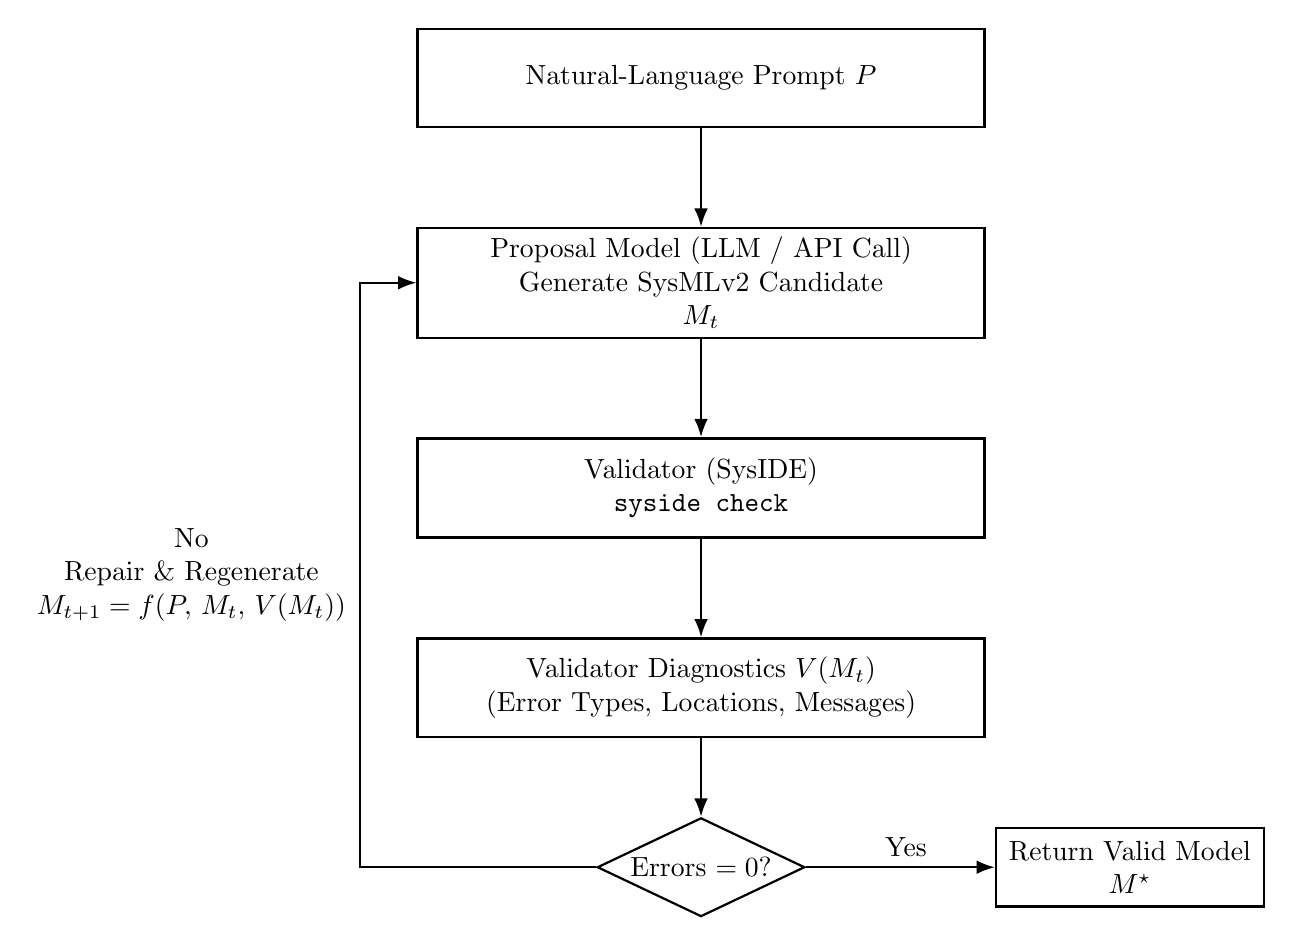
\begin{tikzpicture}[
  box/.style={draw, thick, minimum width=7.2cm, minimum height=1.25cm, align=center},
  oracle/.style={draw, very thick, minimum width=7.2cm, minimum height=1.25cm, align=center},
  decision/.style={draw, thick, diamond, aspect=2.1, inner sep=1.5pt, align=center},
  arr/.style={-Latex, thick},
  looparr/.style={-Latex, thick},
  node distance=1.25cm
]

\node[box] (nl) {Natural-Language Prompt $P$};

\node[box, below=of nl] (llm) {Proposal Model (LLM / API Call)\\Generate SysMLv2 Candidate\\$M_t$};

\node[oracle, below=of llm] (comp) {Validator (SysIDE)\\\texttt{syside check}};

\node[box, below=of comp] (diag) {Validator Diagnostics $V(M_t)$\\(Error Types, Locations, Messages)};

\node[decision, below=1.0cm of diag] (dec) {Errors $=0$?};

\draw[arr] (nl) -- (llm);
\draw[arr] (llm) -- (comp);
\draw[arr] (comp) -- (diag);
\draw[arr] (diag) -- (dec);

\node[box, right=2.4cm of dec, minimum width=3.4cm, minimum height=1.0cm] (done)
  {Return Valid Model\\$M^\star$};
\draw[arr] (dec) -- node[above, xshift=2pt]{Yes} (done);

\draw[looparr]
  (dec.west) -- ++(-3,0)
  |- (llm.west);

\node[align=center]
  at ($(llm.west)!0.5!(dec.west)+(-4,0)$)
  {No\\Repair \& Regenerate\\$M_{t+1}=f(P,\,M_t,\,V(M_t))$};

\end{tikzpicture}
}
\caption{Validator-in-the-loop generate--validate--repair workflow. The prompt is fixed per case, and each revision is driven by deterministic validator diagnostics.}
\label{fig:gcr_loop_methods}
\end{figure}

The production validator oracle is SysIDE validation (\texttt{syside check})~\cite{sensmetry2024syside}. A run is successful and terminates only when zero validation errors are reported.
This oracle choice is additionally supported by an auxiliary ten-case demonstration in the repository showing ANTLR parser pass with production-validation failure, i.e., grammar conformity without operational acceptability~\cite{antlrVsSysideDemo2026}.

\subsection{Dataset, Model Coverage, and Outcome Extraction}
SysMBench provides paired natural-language prompts and ground-truth SysMLv2 models for benchmark evaluation~\cite{jin2025sysmbench}. In this study, we use the curated natural-language prompt set (IDs 1--151) as generation inputs because it was designed to stress SysMLv2 LLM generation across diverse modeling patterns.

To assess model-agnostic behavior of the same controller, we run four model configurations: OpenAI Codex 5.2 (\texttt{gpt-5.2-codex})~\cite{openaiGPT52Codex2026}, Anthropic Sonnet 4.6 (\texttt{claude-sonnet-4-6})~\cite{anthropicSonnet46API2026}, DeepSeek Reasoner (\texttt{deepseek-reasoner})~\cite{deepseekReasonerAPI2026}, and Mistral Large (\texttt{mistral-large-latest})~\cite{mistralLargeLatestDocs2026}. This yields 604 prompt-level cases (151 prompts $\times$ 4 models).

From saved run records, we extract first-shot and eventual pass/fail outcomes, iterations run, iterations to success, unresolved-within-cap status, first/final error counts, cumulative error counts, per-iteration runtime, and token usage. Error families are grouped from validator diagnostics (for example, parsing and reference errors), while warnings are tracked separately and do not change pass/fail labels.

\subsection{Endpoints and Statistical Analysis}
The primary endpoint is production validation acceptance. We report first-shot pass rate, eventual pass rate, unresolved rate, absolute gain (percentage-point difference between eventual and first-shot pass rates), and relative gain:
\[
\frac{p_{\mathrm{final}} - p_{\mathrm{first}}}{p_{\mathrm{first}}}.
\]

Because baseline and pipeline outcomes are paired binary observations on the same prompt--model unit, we test differences with McNemar's test using discordant counts $(b,c)$~\cite{mcnemar1947samplingError}. We use the exact two-sided variant when $b+c\leq 25$ and the continuity-corrected asymptotic variant otherwise, following matched-pairs guidance~\cite{fagerland2013mcnemar}.

We summarize iterations-to-success with mean, median, standard deviation, quantiles, and maximum. Proportion confidence intervals are Wilson 95\% score intervals~\cite{wilson1927probableInference}. Uncertainty in mean iterations-to-success is estimated with a bootstrap 95\% confidence interval (10{,}000 resamples; fixed seed 20260220). These choices align with significance-focused reporting in recent LLM evaluation studies~\cite{cheng2026systemPrompts,lee2025clinicalTrialLlm,wind2025radiologyQa,roberts2024grab}.

All claims are limited to syntactic production-validation acceptance. We do not infer semantic adequacy, behavioral correctness, or design quality from these outcomes.

\subsection{Reproducibility}
All code, run artifacts, and analysis outputs used in this study are stored in the project repository~\cite{sysmbenchCompilerLoopRepo2026}. The repository includes the scripts required to regenerate campaign statistics, tables, and figures.


\section{Results}

\subsection{Overall Production-Validation-Gated Syntactic Outcomes}
Across all 604 prompt-level trials (151 prompts for each of four models), first-shot production validation succeeded for 309/604 cases (51.16\%; 95\% Wilson CI: 47.18--55.13\%). Under validator-in-the-loop refinement, eventual production validation succeeded for 604/604 cases (100.00\%; 95\% Wilson CI: 99.37--100.00\%). The absolute gain from baseline single-shot to final pipeline output was 48.84 percentage points (relative gain 95.47\%), with zero unresolved prompts.

A paired baseline-vs-pipeline test showed a strong shift toward success (McNemar: $b=0$, $c=295$, $p=1.10\times10^{-65}$), indicating that improvements were driven by first-shot failures that were recovered by iterative repair.


\subsection{Per-Model Syntactic Reliability}
All models reached 151/151 eventual production validation under the validator-gated loop, but first-shot pass rates differed substantially. Anthropic Sonnet 4.6 had the highest first-shot pass rate (82.78\%), while OpenAI (41.72\%), DeepSeek Reasoner (41.06\%), and Mistral Large (39.07\%) showed similar first-shot behavior and correspondingly larger iterative gains.


\subsection{Iteration and Recovery Dynamics}
Iterations-to-success over all successful runs had mean 1.733, median 1, and maximum 11 (bootstrap 95\% CI for mean: 1.654--1.816). The distribution was concentrated in early iterations: 309 cases succeeded at iteration 1, 201 at iteration 2, and 60 at iteration 3; only two cases required more than five iterations.

Among first-shot failures, recovery was complete: 295/295 (100\%) failed-first-shot cases eventually passed production validation. For this recovery subset, mean iterations-to-success was 2.502 (median 2, max 11).


\subsection{Production Validator Error Taxonomy}
At first iteration, the dominant error families were \texttt{parsing-error} (1142), \texttt{reference-error} (559), and \texttt{port-definition-owned-usages-not-composite} (82). Across all iterations, the same families remained dominant, with cumulative counts 1658, 794, and 97 respectively.


\subsection{Prompt-Level Difficulty and Diagnostic Burden}
Error burden was heterogeneous across prompts. The largest pooled cumulative error volumes were observed for prompt IDs 93 (133), 9 (88), 139 (81), and 144 (80), indicating a long-tail of syntactically difficult cases even under eventual convergence.


\subsection{Runtime and Token Sensitivity (Secondary)}
Runtime and token data, where available in artifacts, indicate substantial efficiency differences by model despite identical syntactic endpoints. Mean wall-time ranged from 12.97~s (Mistral Large) to 90.45~s (DeepSeek Reasoner), and mean total tokens ranged from 1795.24 to 5938.80 per prompt.

These are secondary operational diagnostics and are not used as primary efficacy claims in this paper.


\section{Discussion}
We discuss why deterministic validator diagnostics provide an effective supervision signal for new, sparsely represented languages like SysMLv2, and the resulting trade-offs in runtime and number of iterations.

\section{Conclusion}
We present a reproducible pathway for reliable natural-language to SysMLv2 translation by embedding deterministic production-validator feedback into LLM generation, thereby guaranteeing syntactically valid, production-validator--accepted output by construction.

\appendix
\section{Auxiliary Demonstration: Grammar Parsability vs. Production Validation}
\label{appendix:antlr_vs_syside}

To support the design choice of using production validation (rather than grammar parsing alone) as the acceptance oracle, we ran an auxiliary demonstration included in the repository under \texttt{experiments/antlr\_vs\_syside/}~\cite{antlrVsSysideDemo2026}. This demonstration is not a second primary experiment; it is a construct-validity check showing that parser acceptance and production acceptance are distinct outcomes.

We evaluated 10 intentionally distinct SysMLv2 examples in \texttt{examples/mismatch\_10\_distinct/}. Each file was designed to remain grammar-parseable while violating a model-wide constraint typically enforced by a production validator. The evaluation pipeline was:
\begin{enumerate}
    \item ANTLR parse check (third-party SysML parser integration in the repository).
    \item Production validation check using SysIDE.
\end{enumerate}

Results were unambiguous: all 10/10 examples passed ANTLR parsing, while 0/10 were accepted by production validation (10/10 mismatch cases). Validator diagnostics were dominated by unresolved-reference failures (9/10, \texttt{reference-error}), with one invocation-typing failure (1/10, \texttt{invocation-expression-instantiated-type}). This pattern directly illustrates that context-free syntax conformance is necessary but not sufficient for operational model acceptance in production modeling environments.

\begin{table*}[t]
\centering
\caption{Ten-case auxiliary demonstration: all examples parse under ANTLR, none pass production validation.}
\label{tab:antlr_vs_syside_10cases}
\begin{tabular}{p{0.17\textwidth} p{0.37\textwidth} p{0.16\textwidth} p{0.16\textwidth}}
\toprule
\textbf{Example ID} & \textbf{Injected Condition} & \textbf{ANTLR Parse} & \textbf{Production Validation} \\
\midrule
01 & Missing imported namespace & Pass & Fail (\texttt{reference-error}) \\
02 & Missing port type & Pass & Fail (\texttt{reference-error}) \\
03 & Missing attribute type & Pass & Fail (\texttt{reference-error}) \\
04 & Missing specialization base & Pass & Fail (\texttt{reference-error}) \\
05 & Action typed by undefined behavior type & Pass & Fail (\texttt{reference-error}) \\
06 & Invocation target is not a behavior & Pass & Fail (\texttt{invocation-expression-instantiated-type}) \\
07 & Missing referenced feature in expression & Pass & Fail (\texttt{reference-error}) \\
08 & Missing root-qualified namespace & Pass & Fail (\texttt{reference-error}) \\
09 & Redefinition of missing feature & Pass & Fail (\texttt{reference-error}) \\
10 & Missing namespace in type use & Pass & Fail (\texttt{reference-error}) \\
\bottomrule
\end{tabular}
\end{table*}



\section*{Acknowledgments}

\bibliographystyle{asmeconf}
\bibliography{references}

\end{document}
